\section{Challenges Of \spath Caching}\label{sec:competitors}

In this section we qualify the differences between static (no change in cache content at service runtime) and dynamic caching (Cache content is changed at service runtime) of \spathsns. We also introduce our state of the art competitor and explain why it is not an adequate solution for the \spath caching problem.


Using a dynamic cache\footnotemark and calculating the utility of each path is very expensive. If a dynamic cache is used, and we want to ensure it always keeps the most useful paths in the cache, it will be very expensive to calculate the utility of a new query with respect how much it overlaps with existing \spaths (i.e. how many vertices it shares with an existing \spathns) and how likely it will be able to answer a query in the future, thus adding a substantial overhead to query processing. As the utility of a \spath is so expensive to calculate, while the \spath service is running, it 
violates goal \ref{item:goal2} in section \ref{subsec:goals}.
\footnotetext{Every time a new query is submitted we consider evicting an old item from the cache and inserting the new query, using a replacement policy e.g. \lru}

Using \lru as the cache replacement policy in a dynamic cache ensures that only minimal overhead is added by using a dynamic cache. When a new query is submitted \lru evicts the least recently used \spath and keeps the most recently used \spaths in the cache.
\lru, however, has several shortcomings: 
\begin{itemize}
\item It has no way to determine the usefulness of inserting a path (i.e. no scoring function), which violates goal \ref{item:goal3} (Sec. \ref{subsec:goals}). Because \lru does not have a scoring function then, even if a path $SP$ is valuable (covers many potential queries), if a sequence of consecutive queries, which $SP$ can not cover, is submitted, then P will be evicted. 
\item \lru also does not have any way to optimize utilization of the cache space available, possibly wasting a lot of space. 
\item If no additional structure is added then querying the cache may require a scan of all paths in the cache to examine the cache can answer a query or not.
\item \lru does not consider utilization of the space in the cache.
\end{itemize}



To give an example of \lrus shortcomings we assume a cache of size 10 (i.e. has space for 10 vertices), using \lruns, and running on the map from figure \ref{fig:rxmap}. Queries Q1-Q6 from table \ref{tab:queries} are used, Q1 first and Q6 last.

The answer to Q1 and Q2 (table \ref{tab:queries}) are added to the cache as both results have a length of 5 and they can both fit. 

Q3 results in a cache hit with Q1. Q1 can answer Q3 because both start and target node (1 and 4) are on the cached path of Q1. This is a property is given by \oss (Lemma \ref{lem:oss}).

When Q4 is submitted Q2 will be evicted and Q4 inserted. Q2 will be evicted from the cache because no item in the cache can answer Q4, and Q2 is the least recently used.

Q5, which \textit{could} have been answered by Q2, now results in the eviction of Q1 and insertion of Q5 because the cache no longer contains any item able to answer Q5 and Q1 is now the least recently used item.

Q6 is not covered by Q3 or Q5, the current elements in the cache, resulting in a cache miss. Because there are 7 nodes in the cache and Q6:$\{v_3,v_4,v_5,v_6\}$ has 4 nodes, Q3 will be evicted (since it was inserted first) and Q6 inserted. 

The end result is that 30\% of the cache space is wasted and out of the 6 queries only we only resulted in a 1 cache hit. If Q1 and Q2 had been kept in the cache we could have had 3 cache hits. However, keeping Q1 and Q2 also  demonstrates \lrus problem with overlapping paths. Q1 and Q2 are identical except for one node, which waste a lot of space on duplicated nodes. Had we represented each node only once (addressed in section \ref{subsec:cacherepresentatons}) we would be able to fit all nodes in the map in the cache.




\section{Contribution} \label{sec:contribution}

Intro to section \\
Show benefits of a static cache over a dynamic cache.\\
List all advantages of a static cache solution \\
(\textit{Static cache} solves goal 2. has zero maintenance cost after filling the cache.)

explain what will be introduced, which sub-problems are considered, and which subsections presents what.


\begin{table}
\begin{tabular*}{\columnwidth}{|l|p{0.76\columnwidth}|}
\hline
\bf Symbol		& \bf Meaning \\\hline
$Q_{s,t}$		& \spath query from $s$ to $t$ \\\hline
$\chi_{s,t}$		& The frequency of a \spath \\\hline
$\Psi$ 			& The Cache \\\hline
$|SP|$			& Length of a \spath \\\hline
$|\Psi|$		& Number of vertices in the cache \\\hline
$\Phi(sp)$		& The set of all sub-paths in a \spath $sp$ \\\hline
$\Phi^c(\Psi)$		& The set of all unique (sub-)paths in $\Psi$ \\\hline
$\Gamma(\Psi)$		& Calculates the total utility of the content in the cache \\\hline 
$G\mathbf{(V,E)}$ 	& Graph representation of the Map \\\hline 
$\mathbf{V}$ 		& The set of vertices in the Map \\\hline 
WL			& Historical workload \\\hline
\end{tabular*}
\caption{Table of Symbols}
\label{tab:symbols}
\end{table}


\begin{figure}[bht]
  \center
        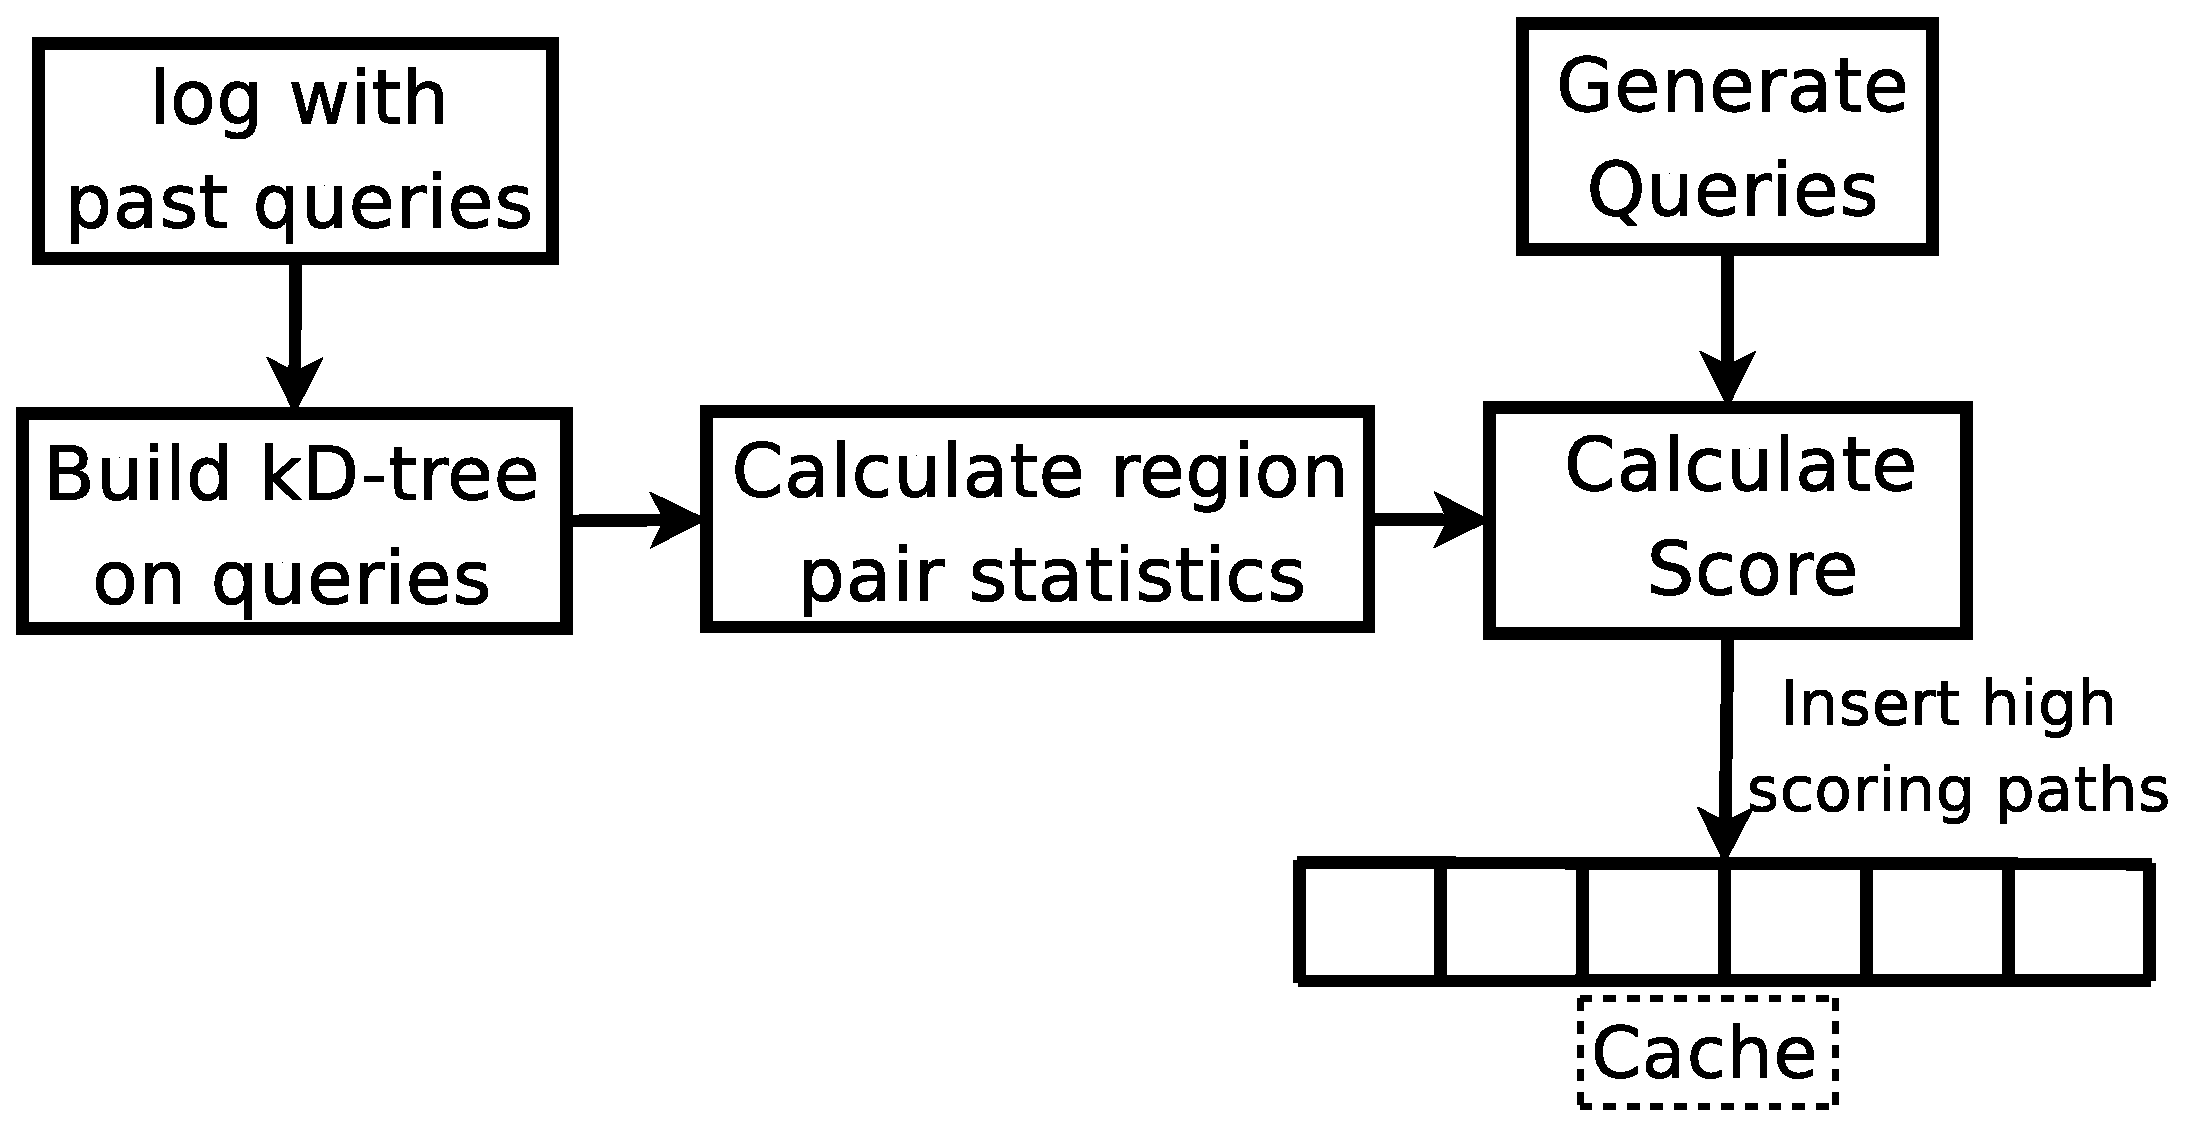
\includegraphics[width=0.5\textwidth]{figures/fillcache}
        \caption{Insertion of cache elements in offline phase.}
  \label{fig:fillcache}
\end{figure}


\subsection{Benefit model}

We will define our goals more formally, introducing the benefit equations we aim to minimize.

A query is a pair of vertices ids $(v_s, v_t)$, denoted $Q_{s,t}$ and the \spath returned from such query we denote $Q_{s,t}$. 
In order to evaluate goal \ref{item:goal3} we calculate the utility of the content in the cache, denoted $\Gamma(\Psi)$. To calculate $\Gamma(\Psi)$ we find the set of unique sub-paths from all \spaths in the cache ($\Psi$) and sum up the frequency, $\chi_{s,t}$, of each unique path.
$\chi$, a table of utility computed from existing historical data. An example of different entries, $\chi_{s,t}$, is given in table \ref{tab:freq}

In order to evaluate our method we try to maximize $\Gamma(\Psi)$ (Eq. \ref{eq:benefit}).



\begin{equation} \label{eq:upsi}
 \Phi^c(\Psi) = \bigcup\limits_{\forall \spath \in \Psi} \Phi(\spath)
\end{equation}

\begin{equation} \label{eq:benefit}
\Gamma(\Psi) = \sum\limits_{SP_{s,t} \in \Phi^c(\Psi)} \chi_{s,t}
\end{equation}

\begin{equation} \label{eq:phi}
\Phi(sp) \leftarrow \{ SP_{s,t} | s \in sp, t \in sp, s \neq t\}
\end{equation}

\begin{table}
\center
\begin{tabular}{|l|l|l|}\hline
Query	&	$Q_{s,t}$	& $SP_{s,t}$ \\\hline 
Q1	&	$Q_{1,6}$ 	& $\{v_1,v_3,v_4,v_5,v_6\}$\\
Q2	&	$Q_{2,6}$ 	& $\{v_2,v_3,v_4,v_5,v_6\}$ \\
Q3	&	$Q_{1,4}$ 	& $\{v_1,v_3,v_4\}$ \\
Q4	&	$Q_{4,7}$ 	& $\{v_4,v_5,v_7\}$ \\
Q5	&	$Q_{2,5}$ 	& $\{v_2,v_3,v_4,v_5\}$ \\
Q6	&	$Q_{3,6}$ 	& $\{v_3,v_4,v_5,v_6\}$ \\\hline
\end{tabular}
\caption{Example Queries}
\label{tab:queries}
\end{table}


\begin{table}
\begin{tabular}{lcp{0.78\columnwidth}}
$\Phi(SP_{1,6})$ &= 	& $\{SP_{1,3},SP_{1,4},SP_{1,5},SP_{1,6},SP_{3,4},SP_{3,5},$\\
		 &	& $SP_{3,6},SP_{4,5},SP_{4,6},SP_{5,6}\}$ \\
$\Phi(SP_{2,6})$ &=  	& $\{SP_{2,3},SP_{2,4},SP_{2,5},SP_{2,6},SP_{3,4},SP_{3,5},$ \\
		 &	& $SP_{3,6},SP_{4,5},SP_{4,6},SP_{5,6}\}$ \\
$\Phi(SP_{1,4})$ &=  	& $\{SP_{1,3},SP_{1,4},SP_{3,4}\}$ \\
$\Phi(SP_{4,7})$ &=  	& $\{SP_{4,5},SP_{4,7},SP_{5,7}\}$ \\
$\Phi(SP_{2,5})$ &=  	& $\{SP_{2,3},SP_{2,4},SP_{2,5},SP_{3,4},SP_{3,5},SP_{4,5}\}$ \\
$\Phi(SP_{3,6})$ &=  	& $\{SP_{3,4},SP_{3,5},SP_{3,6},SP_{4,5},SP_{4,6},SP_{5,6}\}$ \\\hline
$\Phi^c(\Psi)$ 	 &=  	& $\{SP_{1,3},SP_{1,4},SP_{1,5},SP_{1,6},SP_{3,4},SP_{3,5},$ \\
		 &	& $SP_{3,6},SP_{4,5},SP_{4,6},SP_{5,6},SP_{2,3},SP_{2,4},SP_{2,5},$ \\
		 &	& $SP_{2,6},SP_{4,5},SP_{4,7},SP_{5,7}\}$  \\
\end{tabular}
\caption{$\Phi$ (Eq. \ref{eq:phi}) results for queries in table \ref{tab:queries}}
\label{tab:chi}
\end{table}


\begin{table}
\center
\begin{tabular}{|l||l|l|l|l|l|l|l|}
\textbf{$\chi {^s/_t}$}	& $v_1$	& $v_2$	& $v_3$	& $v_4$	& $v_5$	& $v_6$	& $v_7$ \\\hline
$v_1$			& X	& 0	& 0	& 1	& 0	& 1	& 0	 \\
$v_2$			& 0	& X	& 0	& 0	& 1	& 1	& 0	 \\
$v_3$			& 0	& 0	& X	& 0	& 0	& 1	& 0	 \\
$v_4$			& 1	& 0	& 0	& X	& 0	& 0	& 1	 \\
$v_5$			& 0	& 1	& 0	& 0	& X	& 0	& 0	 \\
$v_6$			& 1	& 1	& 1	& 0	& 0	& X	& 0	 \\
$v_7$			& 0	& 0	& 0	& 1	& 0	& 0	& X	 \\
\end{tabular}
\caption{$\chi_{s,t}$ values for $\Phi^c(\Psi)$ in table \ref{tab:chi}}
\label{tab:freq}
\end{table}



When we want to evaluate the utility of $\Psi$ we first calculate $\Phi(\spath)$ for each \spathns. Table \ref{tab:chi} shows the set of sub-paths from the \spaths for each query Q1-Q6 from table \ref{tab:queries} (we assume all queries fit into the cache). Once we have all the sets of sub-paths from the cache content, we use equation \ref{eq:upsi} to union them together and obtain the set of unique sub-paths in the cache, $\Phi^c(\Psi)$ (see table \ref{tab:chi}). After we have obtained $\Phi^c(\Psi)$, we use equation \ref{eq:benefit} to calculate $\Gamma(\Psi)$, the total benefit we expect to have with the content in $\Psi$. With $\Phi^c(\Psi)$ obtained, using $\chi_{s,t}$ values from table \ref{tab:freq}, $\Gamma(\Psi)$ would be 6 i.e. $\chi_{1,6}+\chi_{2,6}+\chi_{1,4}+\dotsb+\chi_{3,6} = 6$, finding a value in table \ref{tab:freq} for all \spaths of $\Phi^c(\Psi)$ (Tab. \ref{tab:chi}).

When filling the cache, during the offline phase, potential \spath$_{s,t}$ items are scored based the $\chi_{s,t}$-value found using the \spath start and end vertices. The score will be zero if the path is already covered by a path, or sub-path, already present in the cache. If we assume $SP_{1,6}$(Q1) is already in the cache and we are considering to insert either $SP_{2,6}$(Q2) or $SP_{4,7}$(Q4) next, then we first find the entry in table \ref{tab:freq} for each query, and check neither is already covered by the content of $\Psi$, i.e not covered by Q1. The score of Q2 would be 2 and for Q4 it would be 1. In this case we would then insert Q2 as it represents the largest expected benefit if inserted into $\Psi$.

\subsection{Hardness Analysis}
Theoretical analysis showing how hard the problem is to solve for \spath caching.\\
show it is NP-Hard
 

\subsection{Greedy algorithm}
We will here introduce \salgo (Alg. \ref{alg:greedy}), the base idea of our greedy algorithm. First we will explain what each line of \salgo does, where after we will give an example to show how \salgo works on example input.

\salgo takes 4 arguments: $G(V,E)$, the graph representation of a map. $\mathbf{\Psi}$, the cache to be used (it is possible to imagine there could be more than one cache in case the \spath provider serve two disjoint areas like i.e. Europe and Japan). $\mathcal{B}$, the cache budget, states how many nodes $\Psi$ can contain before it is full. $\chi$ specifies the statistical information used by \salgons. 
In \salgons, line 1, we first initialize H as a max-heap. Line 2-3 fills H (utility,\spath) pairs, with utility calculated using equation \ref{eq:score}. 
Equation \ref{eq:score} calculates the score of a \spathns, $sp$, based on the sub-paths of $sp$ which are not already present in the cache (Eq. \ref{eq:usp}).

\begin{equation} \label{eq:usp}
U_{sp} \leftarrow \Phi(sp) \setminus \Phi^c(\Psi)
\end{equation}

\begin{eqnarray} \label{eq:score}
S(\chi, \spath_{b,e}, \Psi) = & \chi_{s,t} | SP_{b,e} \in U_{\spath_{b,e}},\neq t \nonumber \\
			      & \chi_{s,t} \in \chi, s=b, t=e, s 
\end{eqnarray}


Line 4 of \salgo starts looping to fill up the cache, terminating when either the cache is full ($| \Psi | \leq  \mathcal{B}$), when the highest scoring \spath has an utility value of 0 ($key_{max} \neq 0$) (According to lemma \ref{lem:addutil} we can not benefit from \spaths with utility equal to zero), or if there are no \spath candidates left to add to $\Psi$.

In line 5 we assign the pair (utility, \spath) the the highest utility score to $\langle  key_{max},  SP_{max} \rangle$ and remove it from H, the max-heap.

In line 6 we update the utility value, $key_{max}$, to know its true utility in case it has changed due to an \spath insertion.

Line 7-11 Implements a compare-and-update/insert loop, avoiding recalculation of all elements in H every round of the loop in line 4. This is necessary because the basis for calculating utility in equation \ref{eq:score} is all possible paths, except those paths, and their sub-paths, already in the cache ($\Psi$). This means that every time we add a \spath to the cache, the utility of some other candidates are likely to be reduced. The way it works is by comparing $key_{max}$ and key of the top element of H, H.TopKey, (line 7), if $key_{max}$ >  H.TopKey we add its \spath to the cache immediately (line 7-9), else we recalculate $key_{max}$ and add $\langle  key_{max},  SP_{max} \rangle$ back into H (line 10-11). This will in the worst case mean we have to recalculate all elements in H after a \spath insertion in $\Psi$, the cache. However, it is likely that the new (utility,\spath) pair with the highest utility score is still close to the top of H, meaning we save a lot of calculations/time. This works since utility scores can only decrease or stay the same, but never increase.


\begin{lemma}\label{lem:addutil}
The utility of a \spath will, when added to the cache, $\Psi$, always increase the utility of $\Psi$ by exactly the utility of the \spathns:

$S(\chi, \spath, \Psi) = \Gamma(\Psi \cup \{\spath\}) - \Gamma(\Psi)$

\end{lemma}

\begin{proof}

When calculating the utility of a \spath $sp$: $S(\chi, sp, \Psi)$ only the set of sub-paths in $sp$ disjoint from $\Phi^c(\Psi)$ is consider as basis for the calculation. 

As there is no overlap between \spaths forming the basis for the utility of $\Psi$ and the set of \spaths forming the basis for the utility of $sp$, then any positive utility value of $sp$ can only be added to the $\Psi$ utility value. 
\end{proof}


To show an example of how \salgo (Alg. \ref{alg:greedy}) works we assume an empty cache, using $\mathcal{B}=15$, table \ref{tab:chi}, \ref{tab:freq}, and the queries from table \ref{tab:queries}. For clarity we limit our example to show only how it works on the queries Q1-Q6 from table \ref{tab:queries}. We use table \label{tab:steputil} to show the utility of each query after each round of the \salgo (Alg. \ref{alg:greedy}, line 4-11)

In the first round we calculate a score for all possible queries (Alg. \ref{alg:greedy}, line 2-3). Since the cache is empty, a \spath score consist of its frequency from table \ref{tab:freq}, as well as the frequency of its sub-paths. For Q1 this would give a utility of 0+1+0+1+0+0+1+0+0+0 = 3 i.e. the frequency of all the sub-paths from $\Phi(SP_{1,6}$) (Tab. \ref{tab:chi}). The utility for Q2-Q6, as well as all other possible queries, is calculated in the same manner. Only the example queries are shown in table \ref{tab:steputil}, $\dots$ is used to symbolize the remaining possible queries. From round 1 (Tab. \ref{tab:steputil}) we can see that Q1 and Q2 are equal candidates for the first item in the cache. In line 4-8 query result $SP_{1,6}$ (from Q1) is chosen, as indicated by the $| \underline{\overline{42}}|$ in round 1 (Tab. \ref{tab:steputil}) . How to break ties, as with Q1 and Q2, would depend on the individual max-heap implementation. 

In the second round of \salgo (Alg. \ref{alg:greedy}, line 4-11) the cache is now no longer empty and we will run line 4-10 several times to find which \spath now has the highest utility. When we first run line 6 we find Q2 now has a utility of 2 and in line 7 we see the top item in H has an utility 1 (expected utility, since has not been recomputed yet), so in line 11 we push back the \spath ($SP_{max}$) together with its updated utility value of 10. Second time we now pop Q6, since it now has the highest utility value of 32. However, after line 6 it now has a utility of 0, so it will be reinserted into H with its new utility (line 11). Third time around we now pop Q5. After line 6 has a utility of 5, which is still smaller than Q4 in the heap, so we reinsert it (line 11). On the fourth turn we pop Q4 with a utility of 15, and after line 6 an actual utility of 11. However, the top of H also has a utility of 11, but since the utility of Q3 can never get larger, only stay the same or become smaller, we don't have to worry about it and we can goto line 7-9 and insert $SP_{4,7}$ (Q4). The second round almost had us recalculate all the items in H (worst case), however, we were still able to avoid calculating the actual utility of Q3 before we were certain we should insert the \spath of Q4.


Round three works as already seen in round 2. We first consider Q3, which has an actual utility of 0, then we consider Q2, whose utility is unchanged after line 6, so we insert it in round 3.

In round 4 Q5 still has a utility of 7, but after recalculation at line 6 it becomes 0 and the algorithm stops. We never insert a \spath with a utility of 0, since any query it can answer, the cache, $\Psi$, can already answer.

\begin{table}
\center
\begin{tabular}{| l| l| l| l| l|}\hline
\small \backslashbox{Query}{Round} 	& 1 	& 2 	& 3 	& 4 	\\\hline
% Q1: ($SP_{1,6}$)		& \zebox{42} 	& -	& -  	& - 	\\\hline
% Q2: ($SP_{2,6}$)		& 42 	& 10	& \zebox{10}	& - 	\\\hline
Q3: ($SP_{1,4}$)		& 11	& 11	& 0	& 0	\\\hline
Q4: ($SP_{4,7}$)		& 15	& \zebox{11}	& -	& - 	\\\hline
% Q5: ($SP_{2,5}$)		& 26	& 7	& 7	& 0	\\\hline
% Q6: ($SP_{3,6}$)		& 32	& 0	& 0	& 0	\\\hline
$\dots$ & $\dots$ & $\dots$ & $\dots$ & $\dots$ \\\hline
\end{tabular}
\caption{Utility for Q1-Q6 during 4 rounds of \salgo. Boxed in values indicate which items are added to the cache in each round.}
\label{tab:steputil}
\end{table}


\begin{algorithm}[H!bt]
\dontprintsemicolon
\SetVline

\SetKwInOut{Input}{input}\SetKwInOut{Output}{output}\SetKw{Return}{return}

\Input
{

	$G(V,E)$: Graph representation of Map \;
	$\Psi$: The cache \;
	$\mathcal{B}$: Cache budget \;
	
}
\vspace{0.7em}
\tcp{\emph{H Contains the utility score of all possible \spaths in $\mathbf{G(V,E)}$. The \spath is the value $v$ and the utility is the key $k$, $(k, v)$. The heap is sorted on the key.}}
H Initialize Max-Heap \;

\tcp{\emph{Initialially fill H}}

\ForAll{$\spath_{s,t} | s \in V, t \in V, s \neq t$} 
{
    H.push(S$(\chi, \spath_{s,t}, \Psi), \spath_{s,t}$) \;
}


\tcp{\emph{Fill cache}}
\While{$| \Psi | \leq \mathcal{B}$ AND $\spath_{ms}.k \neq 0$ OR $| H | > 0$}
{
	\tcp{\emph{Assign (utility,\spath) pair with the highest utility to $\spath_{ms}$}}
	$ \langle  key_{max},  SP_{max} \rangle \leftarrow$ H.pop() \; 
	\tcp{\emph{Update utility, as previous \spath insertion has changed it}}
	$key_{max} = S(\chi, \spath_{max}, \Psi)$
	\tcp{\emph{H.TopKey() looks at the top (k,v) pair without removing it from the heap}}
	\If{$key_{max} \geq H.TopKey$} 	
	{
	    \If{$( \mathcal{B} - | \Psi | ) \geq | \spath_{max} |$}
	    {
		$\Psi.insert(\spath_{max})$\;
	    }
	}
	\Else
	{
	    H.push(S$(\chi, \spath_{max}, \Psi), \spath_{max}$) \;
	}
}

\caption{\salgons($G(V,E), \Psi, \mathcal{B}$)}
\label{alg:greedy}
\end{algorithm}



\subsection{Statistics}

We have previously introduced the notion of utility and shown how we can use the frequency of \spaths (Tab. \ref{tab:freq}) on a map to calculate the utility of an individual \spathns. 

We will make it clear why assuming a uniform distribution of \spaths is an insufficient strategy to base utility calculations on.

Algorithm \ref{alg:buildstatis} gives a high level overview of how our algorithms works and we will reference it in the following sections when we solve a new problem part.
We will make it clear how we extract the frequency information, the statistics, of \spaths on a map (Alg. \ref{alg:buildstatis},PART1). We will show how we use these statistics in order to generate \spath candidates for insertion to the cache, $\Psi$ (Alg. \ref{alg:buildstatis},PART2).

The extraction of statistics extraction and selection of candidate paths is part E of figure \ref{fig:routequery}.



\begin{algorithm} [H!bt]
\dontprintsemicolon
\SetVline

\SetKwInOut{Input}{input}\SetKwInOut{Output}{output}\SetKw{Return}{return}

\Input
{
$G(V,E), \Psi, \mathcal{B}, WL$
}

\tcp{PART1}
WL - historical workload. i.e start-/end-points of trajectories \;

Build regions on G(V,E) \;

Build the table R - holds the vertex sets for each region \;

use WL with R to build $\chi$ (statistics), using regions. \;

\tcp{PART2}

\ForAll{$(R_s,R_t) | (R_s,R_t) \in \chi$} 
{
    Max-Heap H $\leftarrow$ generate-candidate($\chi, WL$) \;
}

\While{Utility(Max-candidate $\in H) \neq 0$ AND $|\Psi| < \mathcal{B}$ }
{
    Add Max-candidate to $\Psi$ \;

    \tcp{\it empty H and generate a new set of candidates.}
    H.clear \;
    \ForAll{$(R_s,R_t) | (R_s,R_t) \in \chi$} 
    {
	Max-Heap H $\leftarrow$ generate-candidate($\chi, WL$) \;
    }
}

\caption{Build Cache Statistics \& Generate Candidates.}
\label{alg:buildstatis}
\end{algorithm}

\subsubsection{Statistics Extraction}\label{sec:statextract}

%how to extract statistics
%GPS traces
%extract endpoints
%calc SP
%For any two nodes in such SP, insert an entry in "ze table"
%EXAMPLE

The purpose of statistics extraction is to build a frequency table like table \ref{tab:freq}. While we have not yet introduced regions, this essentially corresponds to line 4 in PART1 of algorithm \ref{alg:buildstatis}.

There are two extremes when considering what to build table \ref{tab:freq} from. 
In the first extreme we can assume a uniform distribution of all possible queries ($\chi_{s,t} = \frac{1}{v^2}$), meaning that the \spaths chosen by \salgo for the cache will be evenly distributed over the entire map. Due to the number of possible paths on a map, in the order of $\frac{v^2}{2}$ possible paths on the number of vertices in a map, a uniform distribution will pick too many low quality candidates (\spaths very few users will submit queries for in the future) for the cache. 

The second extreme is to build table \ref{tab:freq} from historical information about user queries, resulting in \salgo only adding paths to $\Psi$ which has been observed in the past (Eq. \ref{eq:chi}). We extracted our set of start- and end-points pairs from the historical workload i.e. previously entered \spath queries. We denote this set $\Omega$. We use $\Omega$ to build table \ref{tab:freq} with $v_1,v_2,\ldots,v_n$ on both column and row, n being the number of vertices in the map, $G(V,E)$. We first initialize all values in the table to zero and then for each pair $(s,t) \in \Omega$ we increment the count in cell $s,t$ and $t,s$ by one.

If historical queries are used we can avoid many low quality \spathsns. We do however need to be sure we have enough historical data since candidates for the cache can only be chosen from the exact member of the set of historical workload. If the historical dataset is not large enough we risk overfitting the cache content to the historical dataset, thereby including low quality \spaths too. Between the two option (Uniformly destribution vs. historical workload), using historical information is the best candidate. We will use historical workload in the remainder of this section.

Using historical queries from table \ref{tab:freq} we collect all the start-/end-pairs into $\Omega$ ($\{(1,6),(2,6),(1,7),(2,7)\}$). We then initialize table \ref{tab:chiex} with all zeros and then add all the pairs from $\Omega$ into table \ref{tab:chiex}

\begin{table}
\center
\begin{tabular}{|l||l|l|l|l|l|l|l|}
\textbf{$\chi {^s/_t}$}	& $v_1$	& $v_2$	& $v_3$	& $v_4$	& $v_5$	& $v_6$	& $v_7$ \\\hline
$v_1$			& X	& 0	& 0	& 0	& 0	& 1	& 1	 \\
$v_2$			& 0	& X	& 0	& 0	& 0	& 1	& 1	 \\
$v_3$			& 0	& 0	& X	& 0	& 0	& 0	& 0	 \\
$v_4$			& 0	& 0	& 0	& X	& 0	& 0	& 0	 \\
$v_5$			& 0	& 0	& 0	& 0	& X	& 0	& 0	 \\
$v_6$			& 1	& 1	& 0	& 0	& 0	& X	& 0	 \\
$v_7$			& 1	& 1	& 0	& 0	& 0	& 0	& X	 \\\hline
\end{tabular}
\caption{$\chi_{s,t}$ values for $\Omega$ pairs from table \ref{tab:queries2} queries.}
\label{tab:chiex}
\end{table}


Once we have inserted all pairs from $\Omega$ into table \ref{tab:chiex} we have finished extracting our statistics, the result of which is table \ref{tab:chiex}.


%------------------------------------------------------------------
%------------------------------------------------------------------


When we generate all possible \spath candidates, or generate \spath candidates from the same data source as the statistics were generated from, there is a high chance of overfitting the \spaths to the statistics. By trying to identify popular regions, in stead of specific paths, we can work at a higher abstraction level and more easily capture the tendencies in the historical workload. A tendency could e.g. be that most people drive from a residential area to an industrial area twice a day for work. If we only look at the raw data we can only see that there are many people sharing some set of edges in their routes, but since people usually live in the own house, or different apartment buildings, their starting and end points will be different and we won't capture that they all are going from (generally) the same place to the same area. Having a higher level understanding of popular regions on the map allows us to insert more paths into the cache which serves as connections between two popular regions.

By dividing the map into partitions we can record the statistics for these partitions in stead of the individual \spathsns. Using the example queries in table \ref{tab:queries2} we can easily see that the 4 queries are almost identical, differing by at most 2 vertices. By using our regular statistics method we only know that $v_3,v_4,v_5$ are very popular, but if we use the map/graph in figure \ref{fig:mappartition} and perform the statistic on the regions in stead, then we get something like table \ref{tab:rchitable}. We still check the frequency for each pair in a 
\spathns, but we now increment a region cell in stead of a vertex cell in \ref{tab:rchitable}. 


\begin{table}
\center
\begin{tabular}{l l}
$Q_{1,6} =$ 	& $\{v_1,v_3,v_4,v_5,v_6\}$\\
$Q_{2,6} =$ 	& $\{v_2,v_3,v_4,v_5,v_6\}$ \\
$Q_{1,7} =$ 	& $\{v_1,v_3,v_4,v_5,v_7\}$ \\
$Q_{2,7} =$ 	& $\{v_2,v_3,v_4,v_5,v_7\}$ \\
\end{tabular}
\caption{Historical workload (WL)}
\label{tab:queries2}
\end{table}


\begin{figure}[bht]
  \center
        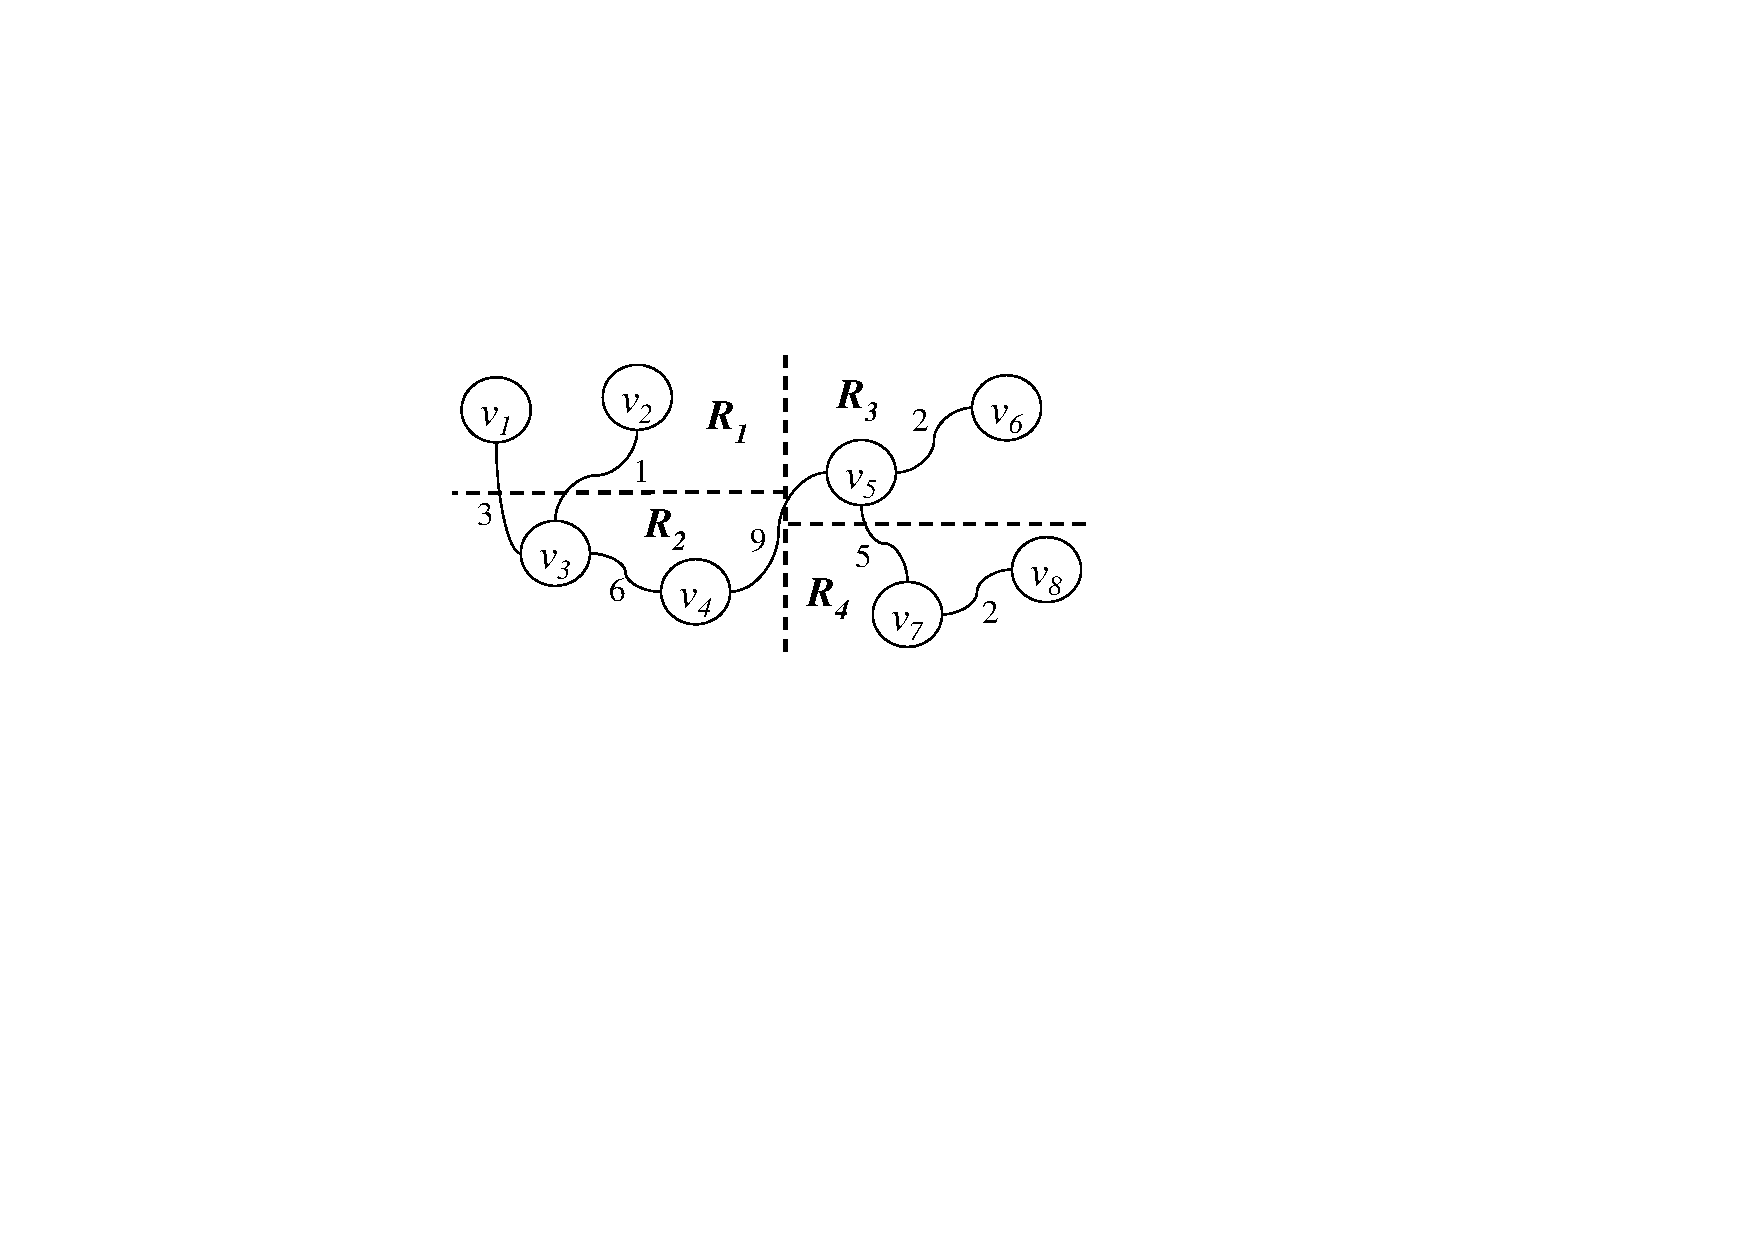
\includegraphics[width=0.45\textwidth]{figures/mappartition}
        \caption{Map Partitioned into 4 areas.}
  \label{fig:mappartition}
\end{figure}

\begin{table}[!Htb]
\center
\begin{tabular}{|l||l|l|l|l|}
\textbf{$\chi {^{R_i}/_{R_j}}$}	& $R_1$		& $R_2$		& $R_3$		& $R_4$\\\hline
$R_1$			& 0		& 0		& 1		& 1 \\
$R_2$			& 0		& 0		& 1	 	& 1 \\
$R_3$			& 1		& 1		& 0	 	& 0 \\
$R_4$			& 1		& 1		& 0	 	& 0 \\
\end{tabular}
\caption{$\chi$ region table produced using query workload from table \ref{tab:queries2}.}
\label{tab:rchitable}
\end{table}


Using the queries in table \ref{tab:queries2} with figure \ref{fig:mappartition} we get the region-to-vertex set relationship in table \ref{tab:vperregion}. Using table \ref{tab:vperregion}, or equivalently equation \ref{eq:rchi}, we can transform the start-/end-pairs into region pairs. Doing this we can build the region version of table \ref{tab:freq} (Tab. \ref{tab:rchitable}). To generate candidates we generate one possible $\Psi$ candidate from each positive entry in table \ref{tab:rchitable} by randomly choosing a start-/end-node from each regions pairs vertex sets i.e. one vertex from each region (Tab. \ref{tab:vperregion}).
Using regions does not change \salgons, regions are only used in the choosing of candidates in line 2 \& 3.
This completes our implementation of line 2-4 of algorithm \ref{alg:buildstatis}


\begin{equation} \label{eq:rchi}
\chi{\tiny _{R_i,R_j}} = | R_i| \times |R_j| \times \chi_{s,t}
\end{equation}

\begin{equation} \label{eq:chi}
\chi{s,t} = \frac{\chi{\tiny _{R_i,R_j}}}{| R_i| \times |R_j|}
\end{equation}



\begin{table}
\center
\begin{tabular}{ll}
$R_1 :$ 	& $\{v_2,v_3\}$\\
$R_2 :$ 	& $\{v_1,v_4\}$ \\
$R_3 :$ 	& $\{v_5,v_7\}$ \\
$R_4 :$ 	& $\{v_6,v_8\}$ \\
\end{tabular}
\caption{Regional vertex sets}
\label{tab:vperregion}
\end{table}

For partitioning the map we use kD-tree, an existing partition method.


%------------------------------------------------------------------
%------------------------------------------------------------------

% % 
\subsubsection{Candidate Generation}

We will explain how and why we chose to implement line 5-6 of algorithm \ref{alg:buildstatis}. Once we have crated the $\chi$-table we need candidate \spaths for insertion into the cache. There are two ways we can generate these candidate. The first way being to generate candidates directly from the map $G(V,E)$, and the second method being based on additional historical workload to produce the candidates.

We can generate candidates for $\Psi$ by finding all possible \spath in $G(V,E)$ as described in algorithm \ref{alg:greedy}. Generating all \spath possible on $G(V,E)$ is quite expensive when considering the possible number of candidates vs. the size of $\mathcal{B}$ which would usually be much smaller. One straight forward optimization to this would be to use only those \spath which has a non-zero entry in table \ref{tab:freq}, this could be very effective if there are few positive values. Another method we can use is sampling, where we just generate a subset of possible candidates. By choosing nodes evenly distributed on the map we can make sure the subset of \spaths picked, still covers the map.

Another way to generate candidates for the cache is to base the candidate generation on historical workload. We modify algorithm \ref{alg:greedy} to take one extra parameter, WL, meaning the historical workload. We replace the requirement in line 2 of algorithm \ref{alg:greedy} to use all possible \spathsns, with a requirement to only calculated the scores on the set of \spaths from WL. The changes to algorithm \ref{alg:greedy} are presented in algorithm \ref{alg:hiscand}.


\begin{algorithm} [H!bt]
\dontprintsemicolon
\SetVline

\tcp{\emph{Initialially fill H}}
\ForAll{$\spath_{s,t} | (s,t) \in WL, s \in V, t \in V, s \neq t$} 
{
    H.push(S$(\chi, \spath_{s,t}, \Psi), \spath_{s,t}$) \;
}

\caption{\salgons($G(V,E), \Psi, \mathcal{B}, \chi, WL$) -- Generating candidates from historical data (Add WL parameter and replaces line 2 \& 3 in algorithm \ref{alg:greedy})}
\label{alg:hiscand}
\end{algorithm}

To generate \spath candidates for $\Psi$ by finding all possible \spath on a map $G(V,E)$ is a relatively simple matter, all we have to do is execute a \spath query for all possible combinations of vertices in $V$, leading to $\frac{|V|^2}{2}$ Candidates.

To restrict the candidate generation to only include those who has a non-zero entry in table \ref{tab:freq} we will exclude any pair of vertices which has an entry of zero in table \ref{tab:freq}. We generate candidates as before, but only consider any pair with a non-zero entry in table \ref{tab:freq}.

If we use sampling we can simply pick random pairs of vertices until we have enough candidates. We assume a uniform random function choosing vertices uniformly distributed on the map, so the sampling method still produce a representative set of candidates covering the map.

Regardless of how the candidates are generated in algorithm \ref{alg:greedy}, it does not affect the main part of the algorithm, only line 2-3. We will be using both sampling from randomly generated candidates as well as split workload. This concludes our implementation of line 5-6 of algorithm \ref{alg:buildstatis}


\subsection{Cache Representations and Cache Concepts} \label{subsec:cacherepresentatons}
The cache storage representation, and the manner in which we search it for cache hits, is crucial to the performance of a cache. We will present the basic, naive, approach as well as several ideas for improvement.
% 
\subsubsection{Simple array of paths}
The simplest way to represent a cache is a simple array of paths (Fig. \ref{fig:cachearray}). This representation is expensive to search since we need to search each individual path in the cache to check for a cache hit. The search procedure is akin to a nested for-loop, every time we want to check if an item is in the cache. We will use this representation as a baseline for comparing optimizations to handle goal \ref{item:goal2} (section \ref{subsec:goals}).

In the example shown in Figure \ref{fig:cachearray} we submit the query $Q_{2,4}$ to the cache (Fig. \ref{fig:cachearray}A). To search the cache we first scan $\Psi_1$ (Fig \ref{fig:cachearray}B) to see if both $v_2$ and $v_4$ are in the cached \spath result \spathns$_{1,3}$. The result is empty so we scan $\Psi_{2}$, which again does not contain $v_2$ and $v_4$, meaning we did not find a cache hit. When we scan $\Psi_3$ we find both $v_2$ and $v_4$, so we stop searching and return the result $\langle v_2,v_3v_4 \rangle$ from $\Psi_3$ (Fig \ref{fig:cachearray}C). Had the result of $Q_{2,4}$ not been in the cache we would have scanned all elements $\Psi_1 - \Psi_6$ before calling a \spath algorithm to calculate the result.

% \begin{itemize}
% \item Short explanation, mention this is naive basic cache representation. 
% \item baseline for goal 2, unoptimized and expensive to use.
% \item main part of explanation carried by example tied to figure.
% \end{itemize}

\begin{figure}[hbt]
  \center
        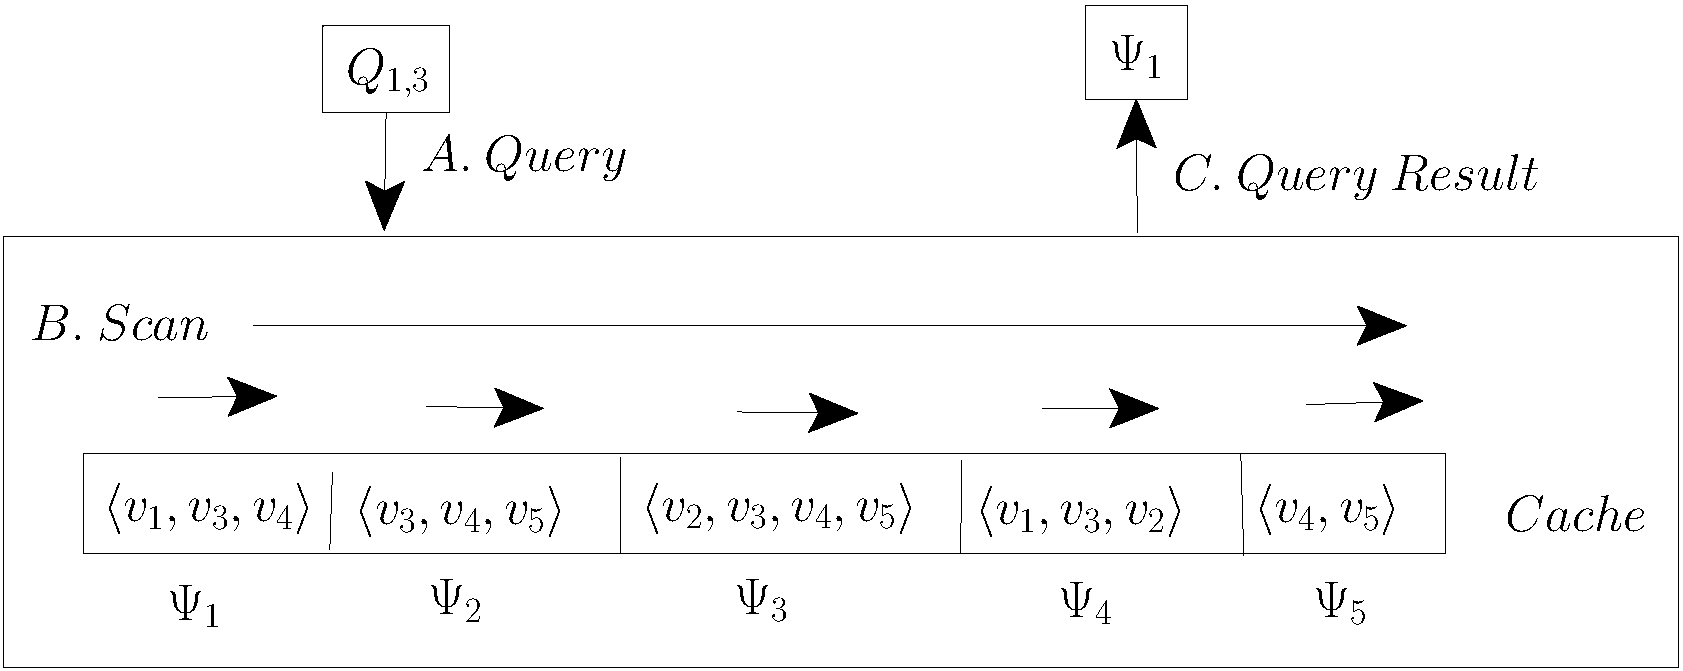
\includegraphics[width=0.45\textwidth]{figures/cachearray.pdf}
        \caption{Simple array of paths.}
  \label{fig:cachearray}
\end{figure}


\subsubsection{Simple array of paths inverted list}
%A simple, yet very effective, way to improve the search time of a cache represented by a simple array is to add an inverted list on top of the cache. We add an inverted list with node ids as keys and values being a list of array indices which holds paths containing specific node ids. By using such an inverted list we just need to do the intersection between the lists retrieved by querying the inverted list with the start and target node ids. 

If we add an inverted list, holding for each vertex a list of paths which includes the vertex in its path (Fig. \ref{fig:cacheinvertlist}), we can reduce the query time notably compared to searching the cache directly. We consider adding an inverted list as it is an effective means to reduce \cet spent on query execution and thereby fulfill goal \ref{item:goal2} from section \ref{subsec:goals}.

In the example shown in figure \ref{fig:cachearray} the start- and end-point of the query $Q_{2,4}$ (Fig. \ref{fig:cacheinvertlist}A) are used to retrieve the list of paths that vertex $v_2$ and $v_4$ are included in (Fig. \ref{fig:cacheinvertlist}B). If the intersection of the two lists are non-empty we have a cache hit. In figure \ref{fig:cacheinvertlist} there are two candidates which can provide the answer, namely $\Psi_3$ and $\Psi_4$. If we have more than one candidate we simply choose the first candidate and return the query answer from that item (Fig. \ref{fig:cacheinvertlist}C).

% 
% \begin{itemize}
% \item refer to previous section and shortly explain how inverted list is used with the array.
% \item mention  - solves goal 2, reduces the query time of the cache.
% \item main part of explanation carried by example tied to figure.
% \end{itemize}

\begin{figure}[hbt]
  \center
        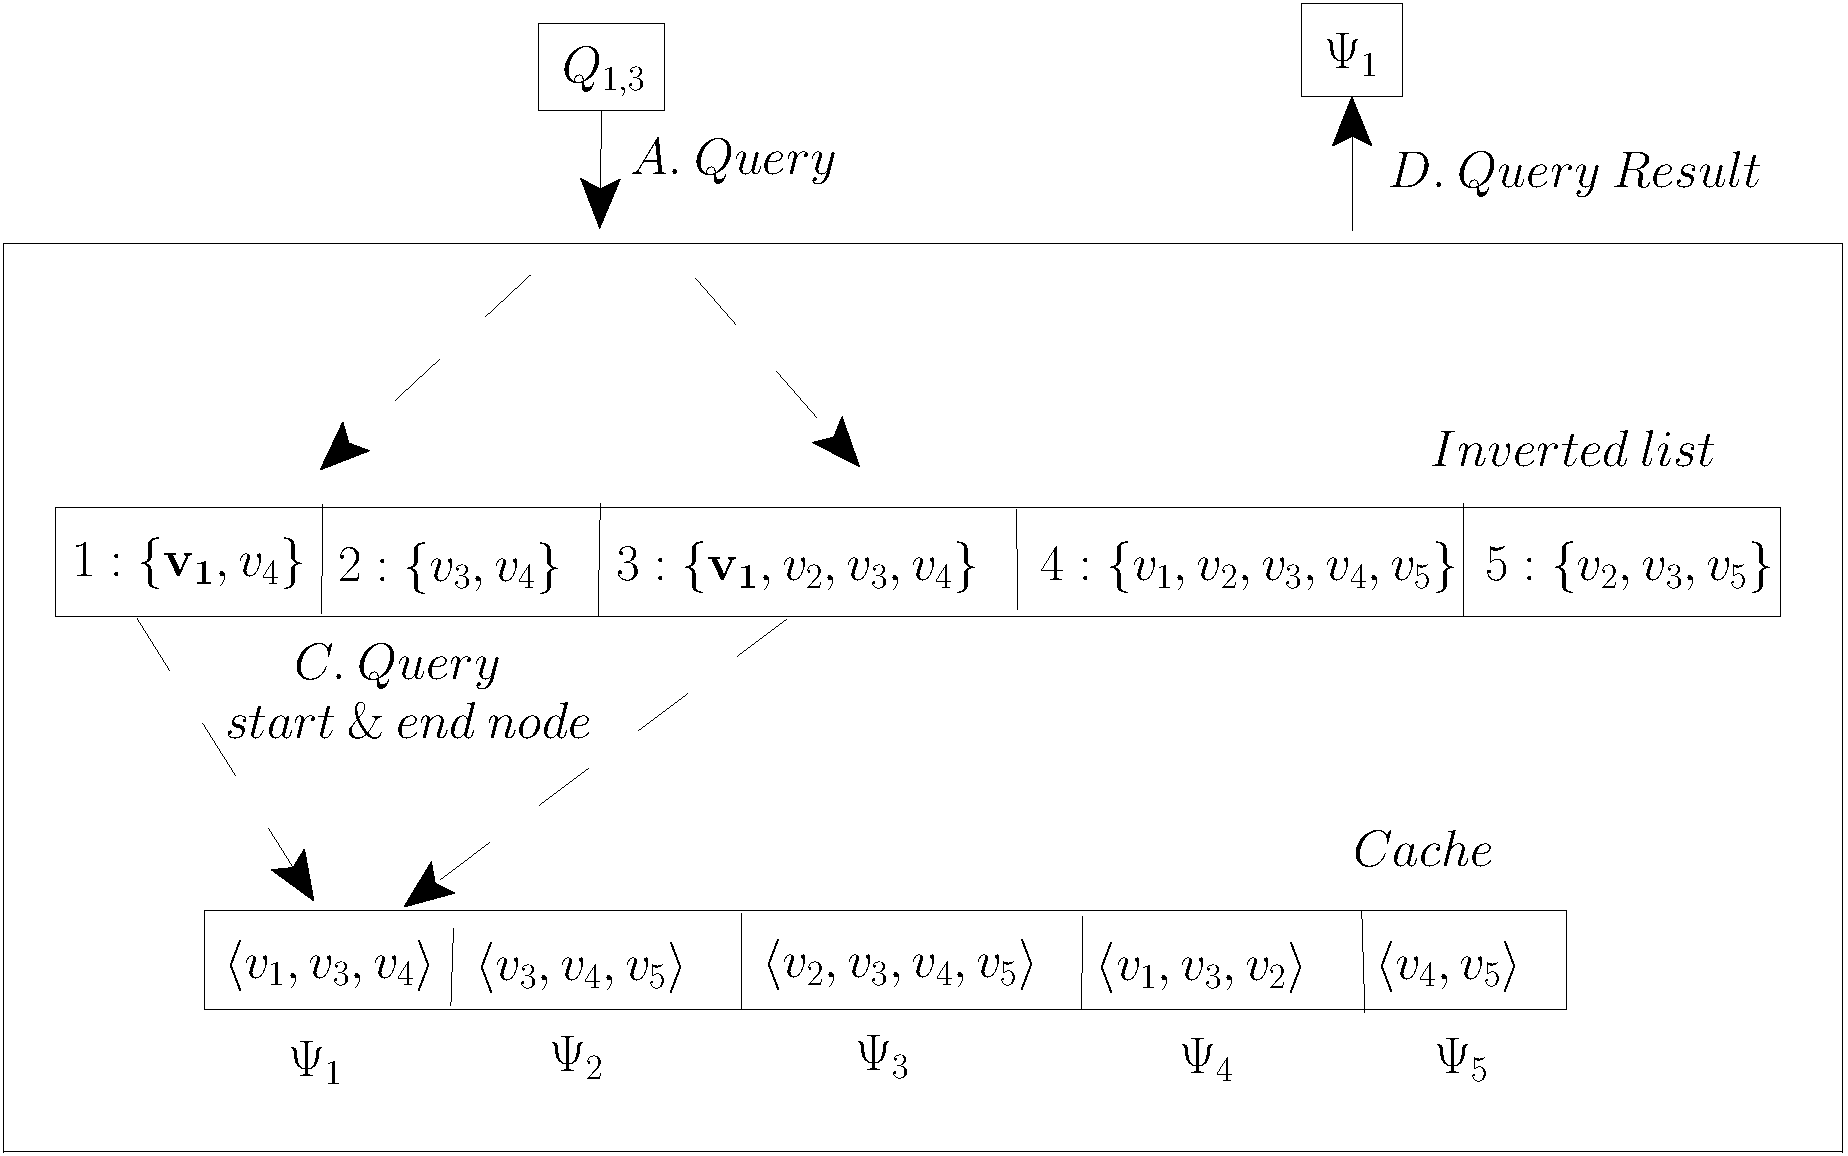
\includegraphics[width=0.50\textwidth]{figures/cachearrayinvertlist.pdf}
        \caption{Simple array of paths, accessed by inverted list.}
  \label{fig:cacheinvertlist}
\end{figure}


\subsubsection{Graph representation \& Sharing sub-paths}% - solves goal 1, allows for more paths in cache, which should translate more cache hits.

An alternative way to represent the cache of \spaths is as a graph (Fig. \ref{fig:cachegraph}). The advantage of representing the cache as a graph is that each vertex is only represented once. We maintain a list of path ids with each vertex, with an entry for each cache item containing the vertex. 
To know whether the cache can answer a query is still easy, simply check whether the intersection of the \spath id set from query's start- and end-vertex is non empty. Finding the actual answer does however take a little more work, as we need to traverse the graph along the \spath query answer to know which vertices are in the list. This searches $\sum_{v_0}^{v_{|\spathns |}} v_i*|e_i|$ vertices, where $v_i \in V$ is a vertex on the \spath answer and $|e_i| \in E $ is the edge degree of $v_i$.

Figure \ref{fig:cachegraph} illustrates how the query $Q_{1,5}$ is queried on the graph representation of the cache. First we check if the \spath id set intersection of $v_1$ and $v_5$ is non-empty (Fig. \ref{fig:cachegraph}B). Since there is a \spath (path 1) in the cache which can answer $Q_{1,5}$, we will do a search for all vertices between $v_1$ and $v_5$ which also includes path 1 in their \spath id set (Fig. \ref{fig:cachegraph}C). The edges taken when doing this search is shown with bold arrows. $v_2$ is also examined since it is connected to the actual path, but is ignored afterwards as $v_2$ does not have \spath id 1 in its set. Note that since both $v_1$ and $v_5$ has id 1 in their \spath id set, then there will always be a path between them. Once we have traversed the graph and found the answer to $Q_{1,5}$ we return the result (Fig. \ref{fig:cachegraph}D).

As the graph representation is very compact and only represents each vertex once, it allows for a high degree of sub-path sharing, which directly translates into more space available for more paths in the cache. As such the goal of this representation is to reduce the overall \cet used on \spath calculation (Goal \ref{item:goal1} in section \ref{subsec:goals}) by increasing the number of paths in the cache so fewer queries may need to be calculated.

The cache query time is slightly worse than when using an array with an inverted list. The graph representation overall fulfills goal \ref{item:goal1} by allowing more paths in the cache, but it does unfortunately also impose some overhead to the query answer time, as each answer needs to be found in the graph (Fig. \ref{fig:cachegraph}C) once it has been confirmed (Fig. \ref{fig:cachegraph}B).

\begin{figure}[hbt]
  \center
        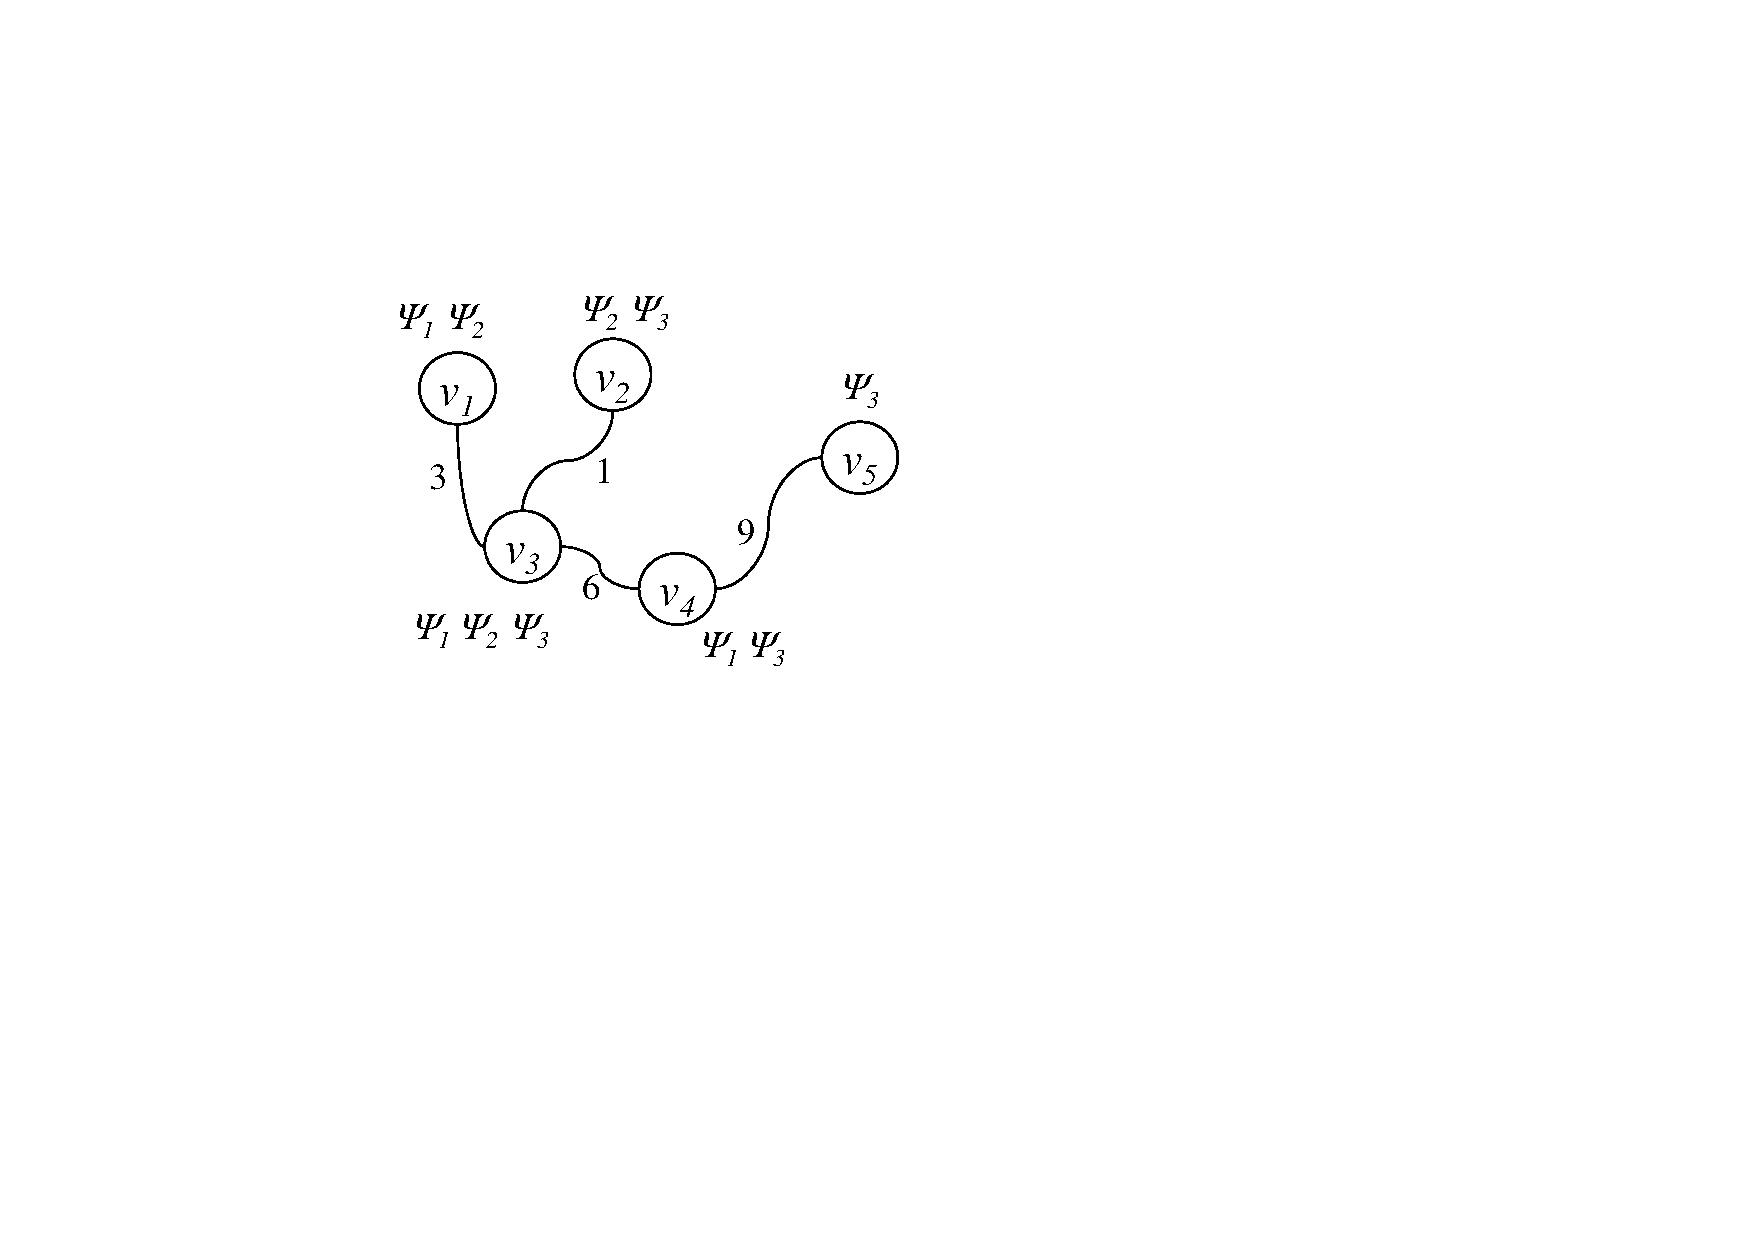
\includegraphics[width=0.45\textwidth]{figures/cachegraph}
        \caption{Graph representation of \spath cache. Inserted paths from table \ref{tab:queries}}
  \label{fig:cachegraph}
\end{figure}

% \begin{itemize}
% \item Explain graph representation.
%     \begin{itemize}
%     \item how are paths represented
%     \item how is the search performance of the cache compared to previous array approach
%     \item solves goal 1, allows for more paths in cache, which should translate more cache hits.
%     \end{itemize}
% \item Explain sub-path sharing.
%     \begin{itemize}
%     \item solves goal 1, allows for more paths in cache, translating to more cache hits. Unfortunately has a negative impact on goal 2 as it introduces some overhead in query time.
%     \item very compact representation
%     \end{itemize}
% \item most of the explanation should be tied to figure \ref{fig:cachegraph}
% \end{itemize}

An optimization to the graph representation is to not directly represent each path id in the path id set of each vertex. We can do this by collapsing each continues sequence of path ids, which then again allow for even more ids to be added to the cache. Table \ref{tab:compressedlist} shows how the id sets for each vertex in figure \ref{fig:cachegraph} can be collapsed and what the savings are in terms of how many more path ids we have space for.




\begin{table}
\center
\begin{tabular}{|l|l|l|}\hline
Vertex 	& Compressed list & Num. path ids saved \\\hline
$v_1$ 	& $\langle 1, 3 \rangle$ 	& 0 \\\hline
$v_2$ 	& $\langle2, 5 \rangle$ 	& 0 \\\hline
$v_3$ 	& $\langle 1-3, 5-6 \rangle$ 	& 1 \\\hline
$v_4$ 	& $\langle 1-6 \rangle$ 	& 4 \\\hline
$v_5$ 	& $\langle 1-2, 4-6 \rangle$ 	& 1 \\\hline
$v_6$ 	& $\langle 1-2, 6 \rangle$ 	& 0 \\\hline
$v_7$ 	& $\langle 4 \rangle$ 		& 0 \\\hline

\end{tabular}
\caption{Compressed list content and the space saved by using them.}
\label{tab:compressedlist}
\end{table}
